\documentclass[12pt]{article}
\usepackage[frenchb]{babel} 
\usepackage[T1]{fontenc}
\usepackage[latin1]{inputenc}
%\usepackage{lmodern} 
\usepackage{graphicx}
\usepackage{multirow}
\usepackage[top=2.5cm, bottom=2.5cm, left=2.5cm , right=2.5cm]{geometry}
%\usepackage{amsmath}
%\usepackage{amsthm}
%\usepackage{amsfonts}
\usepackage{empheq}
\usepackage{setspace}
\usepackage{hyperref}
\hypersetup{pdftitle = {INF8225 - Intelligence Artificielle}, pdfauthor={Maxime Schmitt}}
\usepackage{color}
\usepackage{subfigure}
\usepackage{fancyvrb}
\usepackage{SIunits}
\usepackage{numprint}
\usepackage{enumitem}
\usepackage{calc}
\usepackage{listings}
\usepackage{float}
\usepackage{cellspace}
\usepackage{algpseudocode}
\cellspacetoplimit=4pt
\cellspacebottomlimit=4pt

% ----------------------------------- FANCY HEADER -----------------------------------
\usepackage{fancyhdr}
\pagestyle{fancy}
\renewcommand{\headrulewidth}{0.5pt}
%\fancyhead[C]{\textbf{page \thepage}} 
\fancyhead[L]{}
\fancyhead[R]{Rapport de laboratoire 1}

\renewcommand{\footrulewidth}{0.5pt}
\fancyfoot[C]{\textbf{\thepage}} 
\fancyfoot[L]{Polytechnique Montr�al}
\fancyfoot[R]{INF8225}
% ------------------------------------------------------------------------------------


\providecommand{\e}[1]{\ensuremath{\cdot 10^{#1}}}
\newcommand{\question}{\noindent$\bullet$\;\;}
\newcommand{\eau}{\ensuremath{\text{H}_2 \text{O}}}
\newcommand{\dio}{\ensuremath{\text{CO}_2}}
%\addto\captionsfrancais{\renewcommand{\chaptername}{Labo}}

\definecolor{mygreen}{RGB}{28,172,0} % color values Red, Green, Blue
\definecolor{mylilas}{RGB}{170,55,241}

\begin{document}

\hyphenation{HyperLogLog experimental techno-logy according develop-ment}

\begin{titlepage}
\newcommand{\HRule}{\rule{\linewidth}{0.5mm}} % Defines a new command for the horizontal lines, change thickness here

%-------------------------------------------------------------------------------------
%	LOGO SECTION
%-------------------------------------------------------------------------------------
\raggedright
\center 
\includegraphics[width = 0.33\textwidth]{../../logo}\\[5cm] 
\centering
%-------------------------------------------------------------------------------------
%	TITLE SECTION
%-------------------------------------------------------------------------------------
\HRule \\[0.4cm]
{ \huge \bfseries INF8225 TP3 - Rapport de laboratoire}\\[0.4cm] 
{ \Large \bfseries Apprentissage dans un r�seau de neurones}\\
\HRule \\[1cm]
%-------------------------------------------------------------------------------------
%	AUTHOR SECTION
%-------------------------------------------------------------------------------------

\vspace{\fill}
\begin{center} 
\large
Maxime \textsc{Schmitt}\\
1719088
\end{center}

%-------------------------------------------------------------------------------------
%	DATE SECTION
%-------------------------------------------------------------------------------------
\begin{center}
{\Large \today}
\end{center}
%-------------------------------------------------------------------------------------
\vfill 
\end{titlepage}

%\tableofcontents

\section{2 hidden layers Neural Network optimization}

\begin{algorithmic}[H]
\For{\textbf{each} \textit{theta} in ($\theta_{firstHiddenLayer}$,$\theta_{secondHiddenLayer}$, $\theta_{outputLayer}$)}
	\State $theta[:,:-1] \gets rand()$ \Comment W (without the bias)
	\State $theta[:,-1] \gets 0$ \Comment B (only the bias)
\EndFor
\newline
\While{loss function didn't converge}
	\State Segmentation of the input and output training data in minibatches \textit{miniBatchesInput} and \textit{miniBatchesOutput}
	\For{\textbf{each} (X,Y) in (miniBatchesInput, miniBatchesOutput)}
		\State \textit{\# Feed forward}
		\State Adding a line of 1 at the end of X (bias)
		\State $activation_{firstHiddenLayer} \gets activationFunction(\theta_{firstHiddenLayer} * X)$
		\State Adding a line of 1 at the end of X $activation_{firstHiddenLayer}$ (bias)
		\State $activation_{secondHiddenLayer} \gets activationFunction(\theta_{secondHiddenLayer} * activation_{firstHiddenLayer})$\newline
		\State Adding a line of 1 at the end of X $activation_{secondHiddenLayer}$ (bias)
		\State $activation_{outputLayer} \gets outputActivationFunction(\theta_{outputLayer} * activation_{secondHiddenLayer})$\newline
		
		\State \textit{\# Back propagation}
		\State $\delta_{outputLayer} \gets - (Y - activation_outputLayer)$
		\State $gradientW_{outputLayer} \gets \delta_{outputLayer} * activation_{secondHiddenLayer}[:,:-1]$
		\State $gradientB_{outputLayer} \gets \delta_{outputLayer} * activation_{secondHiddenLayer}[:,-1]$
		\newline
		\State $\delta_{secondHiddenLayer} \gets derivatedActivationFunction(activation_{firstHiddenLayer}) * \theta_{outputLayer} * \delta_{outputLayer}$
		\State $gradientW_{secondHiddenLayer} = \delta_{secondHiddenLayer} * activation_{firstHiddenLayer}[:,:-1]$
		\State $gradientB_{secondHiddenLayer} = \delta_{secondHiddenLayer} * activation_{firstHiddenLayer}[:,-1]$
		\newline
		\State $\delta_{secondHiddenLayer} = derivatedActivationFunction(X) * \theta_{secondHiddenLayer} * \delta_{secondHiddenLayer}$
		\State $gradientW_{firstHiddenLayer} = \delta_{firstHiddenLayer} * X[:,:-1]$
		\State $gradientB_{firstHiddenLayer} = \delta_{firstHiddenLayer} * X[:,-1]$
		\newline
		\State \# \textit{Parameters update}
		\State $\theta_{firstHiddenLayer}[:,:-1] = \theta_{firstHiddenLayer}[:,:-1] - learningRate * gradientW_{firstHiddenLayer}$
		\State $\theta_{firstHiddenLayer}[:,-1] = \theta_{firstHiddenLayer}[:,-1] - learningRate * gradientB_{firstHiddenLayer}$
		\newline
		\State $\theta_{secondHiddenLayer}[:,:-1] = \theta_{secondHiddenLayer}[:,:-1] - learningRate * gradientW_{secondHiddenLayer}$
		\State $\theta_{secondHiddenLayer}[:,-1] = \theta_{secondHiddenLayer}[:,-1] - learningRate * gradientB_{secondHiddenLayer}$
		\newline
		\State $\theta_{outputLayer}[:,:-1] = \theta_{outputLayer}[:,:-1] - learningRate * gradientW_{outputLayer}$
		\State $\theta_{outputLayer}[:,-1] = \theta_outputLayer[:,-1] - learningRate * gradientB_{outputLayer}$
	\EndFor
\EndWhile
\end{algorithmic}

\section{Experiments and hyper parameters optimization}

\subsection{Considered parameters}

The hyper parameters that we can change are :
\begin{itemize}
	\item \textbf{batchNumbers}: Number of mini batches to use
	\item \textbf{learningRate}: Learning rate of the network
	\item \textbf{activationParameter}: Value of the coefficient for the
	piecewise linear activation function
	\item \textbf{WInitValue}: Maximal initial value for the random
	initialization of $\theta$
	\item \textbf{convergenceThreshold}: value that determines when we
	consider that the loss function has converged
	\item \textbf{hiddenLayersNumber}: Number of hidden layers in the network
	\item \textbf{firstHiddenLayerSize}: Number of nodes in the first hidden
	layer
	\item \textbf{secondHiddenLayerSize}: Number of nodes in the second
	hidden layer (when applicable)
\end{itemize}

Experimentally, we found that the following values for these parameters made
a good combination :
\begin{itemize}
	\item \textbf{batchNumbers} = 5000
	\item \textbf{learningRate} = 0.01
	\item \textbf{activationParameter} = 0.01
	\item \textbf{WInitValue}: 0.1
	\item \textbf{convergenceThreshold}: 0.01
	\item \textbf{hiddenLayersNumber}: 1 or 2
	\item \textbf{firstHiddenLayerSize}: 300
	\item \textbf{secondHiddenLayerSize}: 100 (when applicable)
\end{itemize}

Note that this set doesn't necessarily provide the best result but it
provides a good result while not requiring too much time to run and was
chosen considering these two critera.

\subsection{Comparison of one and two hidden layer networks}

In this section, we provide the results and the learning curves for the
networks using the parameters given previously, the two only differing from
each other with the number of hidden layers they contain :
\begin{itemize}
	\item The first network contains only one hidden layer of 300 nodes
	\item The second network contains two hidden layers : the first one of
	300 nodes and the second one of 100 nodes
\end{itemize}

On the figure~\ref{hidden2} and figure~\ref{hidden1} we can see respectively
the learning curves of the network with 2 hidden layers and with 1 hidden
layer.

At the end we also have the following accuracies on the testing:\\
97.03\% for the network with two hidden layers
97.4\% for the network with one hidden layer

The least deep seems to provide a better resutl, but we can imagine that with
some finer parameters tuning we could be able to get better results with
the deepest one, especially considering that our current parameters converge
in only 8 iterations.

\begin{figure}[H] 
	\centering
	\subfigure[Accuracy on the training and the validation sets]{
		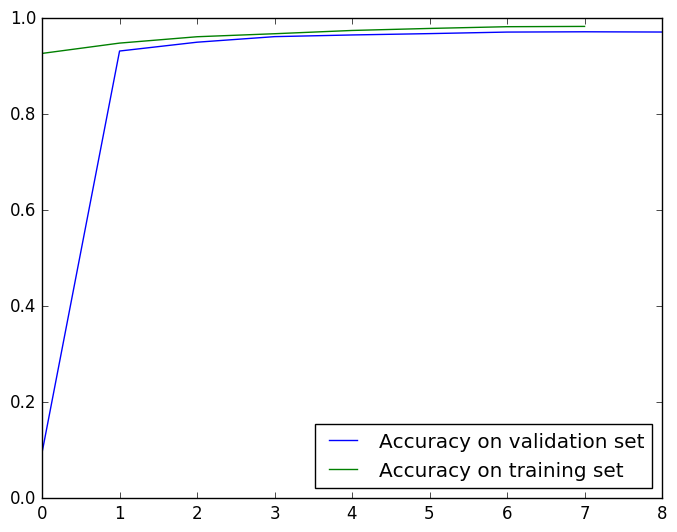
\includegraphics[width = 0.75\textwidth]{images/accuracy2.png}
		\label{accuracy2} }
	\quad
	\subfigure[Loss function]{
		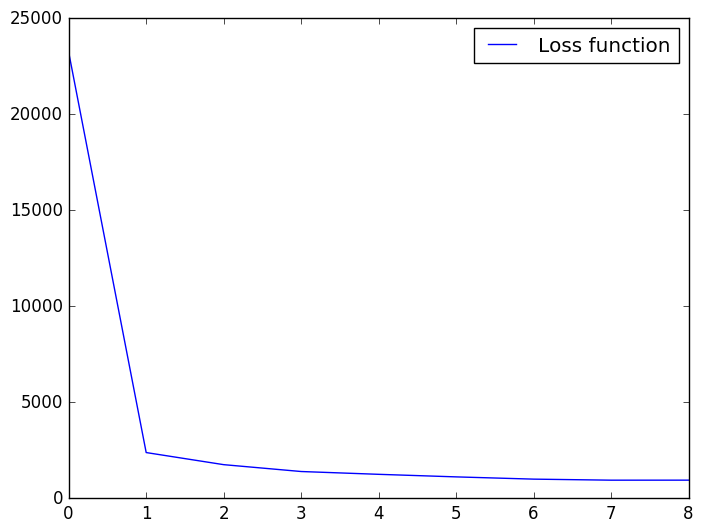
\includegraphics[width = 0.75\textwidth]{images/lossFunction2.png}
		\label{lossFunction2} }
	\caption{Curves for the network with two hidden layers} 
	\label{hidden2}
\end{figure}

\begin{figure}[H] 
	\centering
	\subfigure[Accuracy on the training and the validation sets]{
		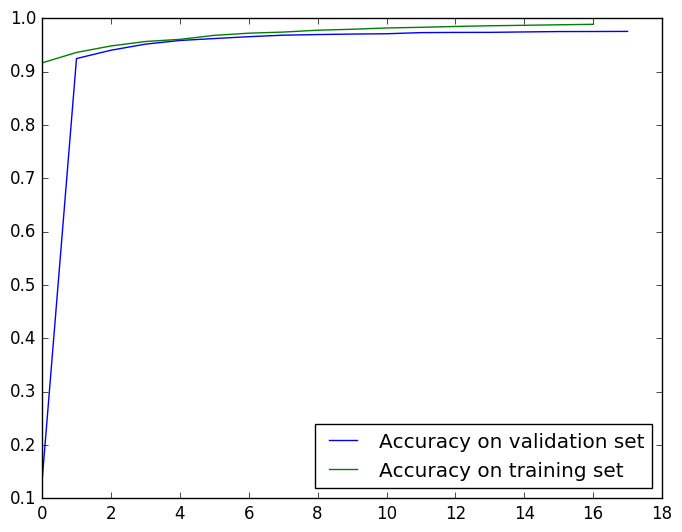
\includegraphics[width = 0.75\textwidth]{images/accuracy1.png}
		\label{accuracy1} }
	\quad
	\subfigure[Loss function]{
		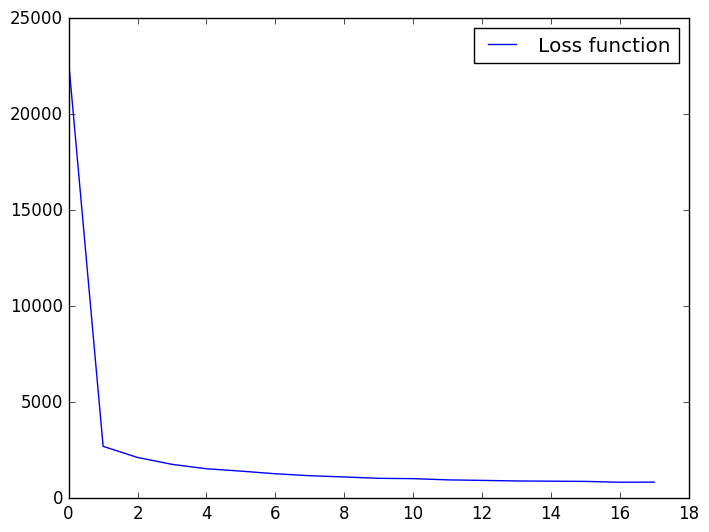
\includegraphics[width = 0.75\textwidth]{images/lossFunction1.png}
		\label{lossFunction1} }
	\caption{Curves for the network with one hidden layer} 
	\label{hidden1}
\end{figure}


\section{Conclusion}

With this work, we succeeded in implementing a multi-layer neural network
and made some experiment to get some intuition on the influence of the
various parameters on the result of the learning, and compared two networks
of different deepness. However this comparison is quite simplistic and a more
thourough study should be done to obtain a clear result.

Moreover, the proposed implementation could be improved by adding a
regularization term to the learning, to avoid some overfitting and therefore
get better results on the testing data set at the end of the learning phase.

\end{document}




























